\documentclass[11pt]{article}
\usepackage{graphicx}
\usepackage{listings}
\usepackage{anysize}
\renewcommand{\topfraction}{0.9}    % max fraction of floats at top
\renewcommand{\bottomfraction}{0.8}
\marginsize{2cm}{2cm}{1cm}{2cm}
\lstset{
  language=C,                     % choose the language of the code
}
\begin{document}

\title{Algorithms Coursework}
\author{Xueqi Chen and Haixiao Su}

\maketitle
\section{Randomised Algorithms}
The below figures indicates the changes in time/number of executions in proportional to the size of the words added into the set for three different randomised algorithms: Skip List, Bloom Filter and Randomised BST. The observed trend for time complexity for Skip List and Bloom Filter all follows the similar pattern, which is predicted to be O(log n). \\
We have generated some graphs to demonstrate this trend. This is done by using the provided analyse program, and provide relevant numbers such as numbers to repeat and number of words to add. Two graphs are generated this way, one is for Set Size and Counter Value, which is the number of times that a function is called. The Counter Value is incremented at the beginning of the functions to be recorded. The second graph is for Set Size and Mean Execution Time, this is calculated by operating on the same set of data each time, and repeating this operating several times would give a more accurate result. When we were testing, we tested the set size of 500, and repeated this process 5000 times to ensure the accurancy of the result.
\section{Add}
\begin{figure}[ht]
\centering
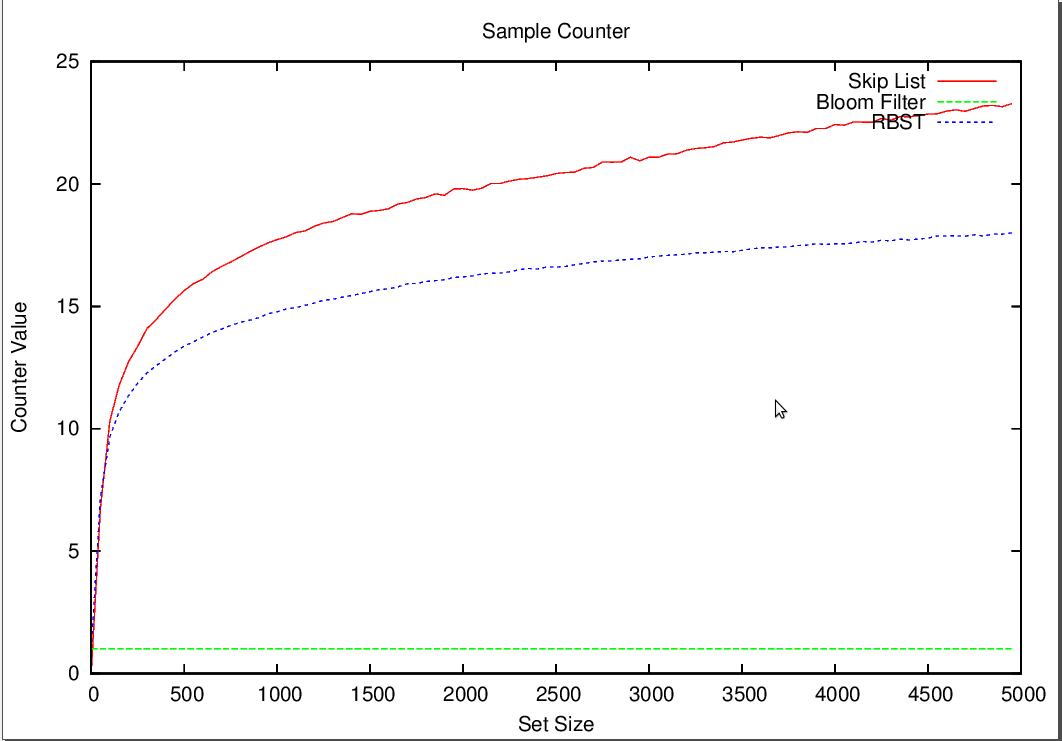
\includegraphics[height=70mm,width=100mm]{addcounter.png}
\caption{addcounter}
\end{figure}
\begin{figure}[ht]
\centering
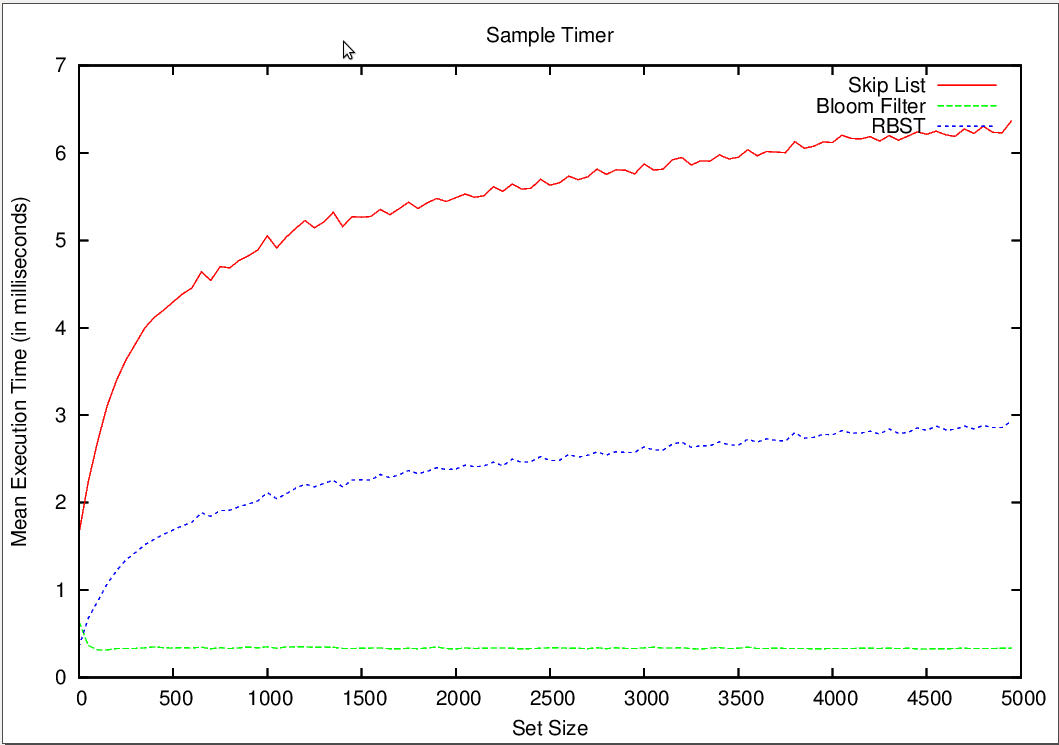
\includegraphics[height=70mm,width=100mm]{addtimer.png}
\caption{addtimer}
\end{figure}

For the Bloom Filter, the complexity is constant, as Bloom Filter itself is a Hash Table. 

\section{Delete}
\begin{figure}[ht]
\centering
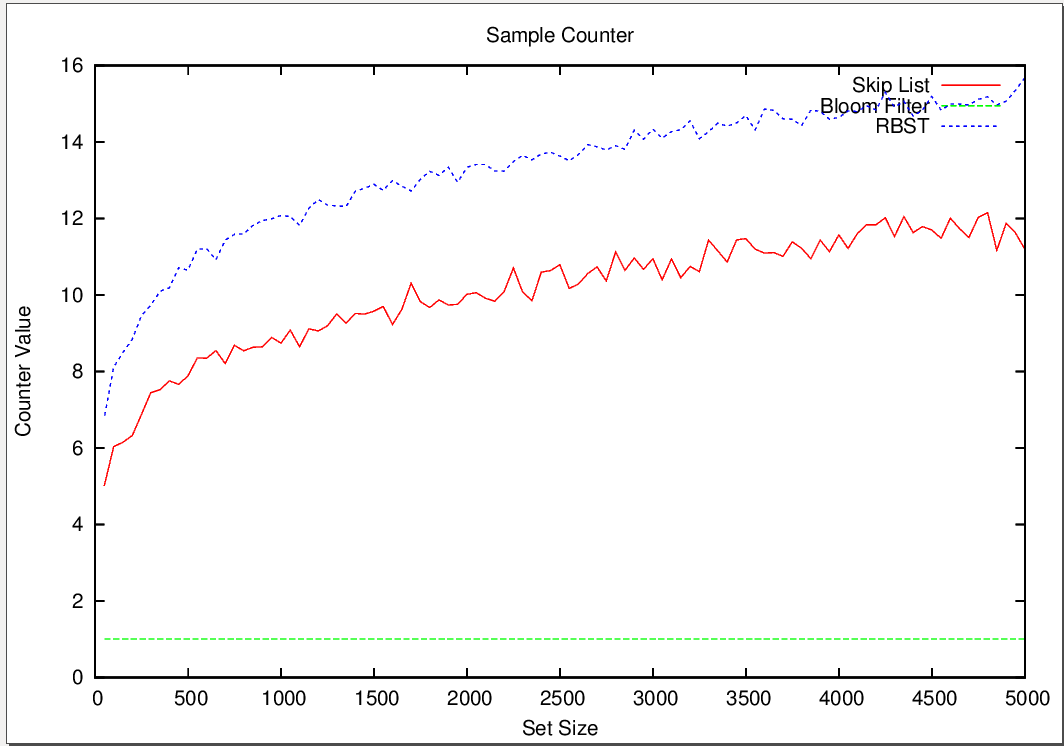
\includegraphics[height=70mm,width=100mm]{delcounter.png}
\caption{delcounter}
\end{figure}
\begin{figure}[ht]
\centering
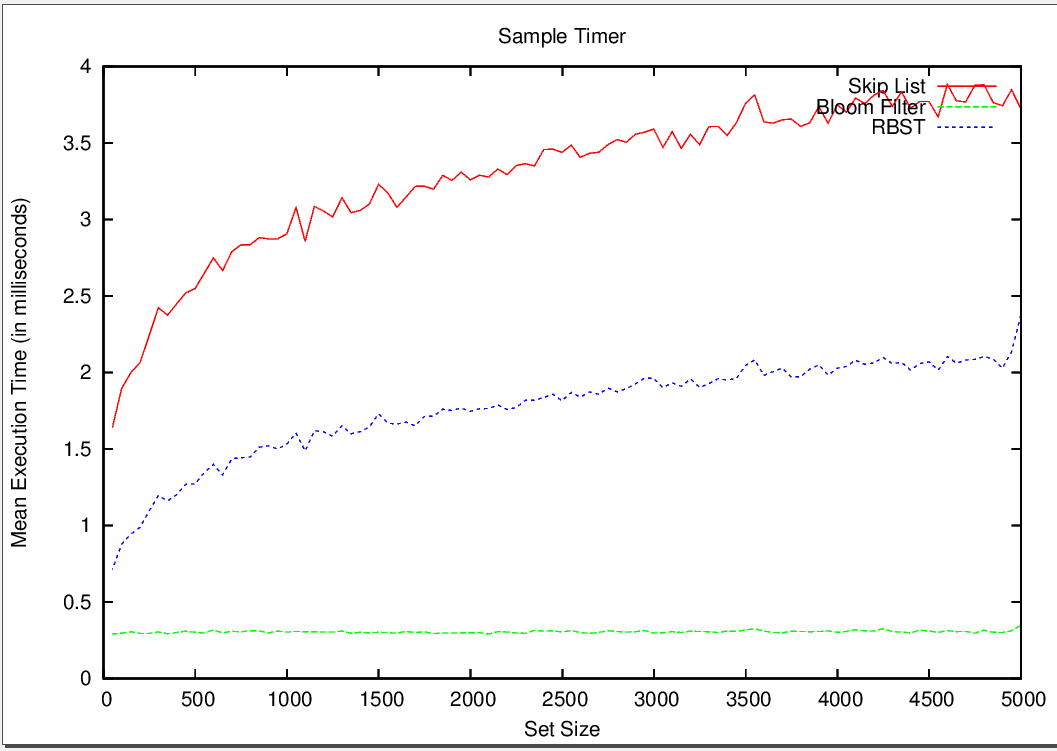
\includegraphics[height=70mm,width=100mm]{deltimer.png}
\caption{deltimer}
\end{figure}



\section{Find}
\begin{figure}[ht]
\centering
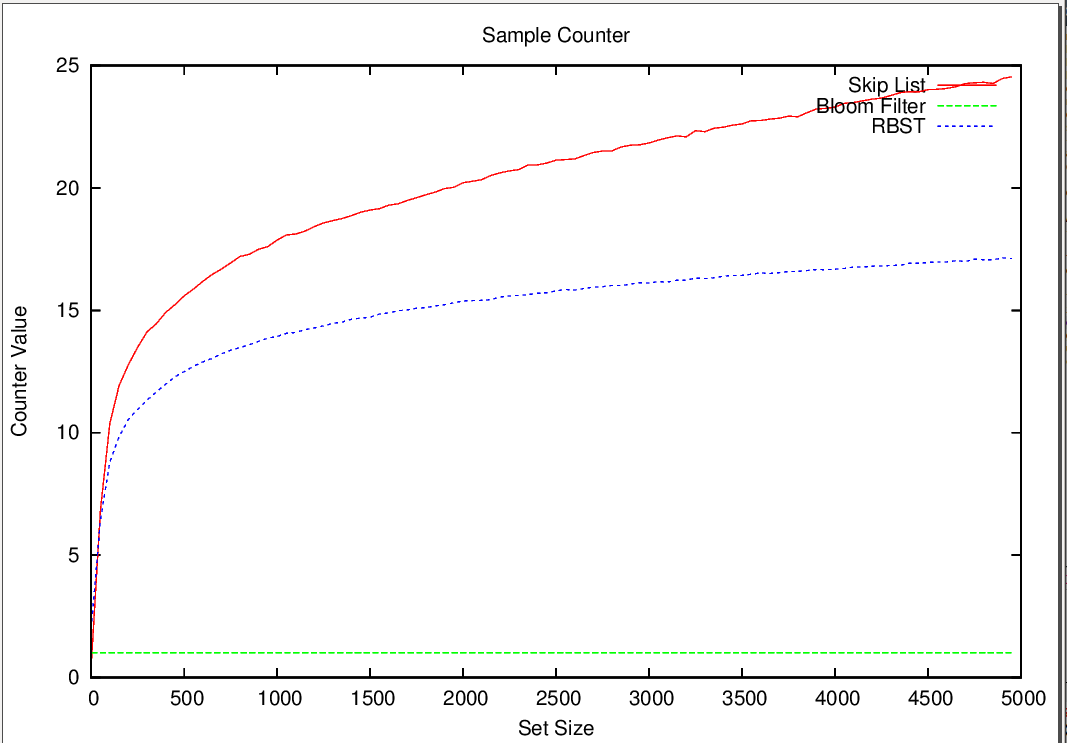
\includegraphics[height=70mm,width=100mm]{findcounter.png}
\caption{findcounter}
\end{figure}
\begin{figure}[ht]
\centering
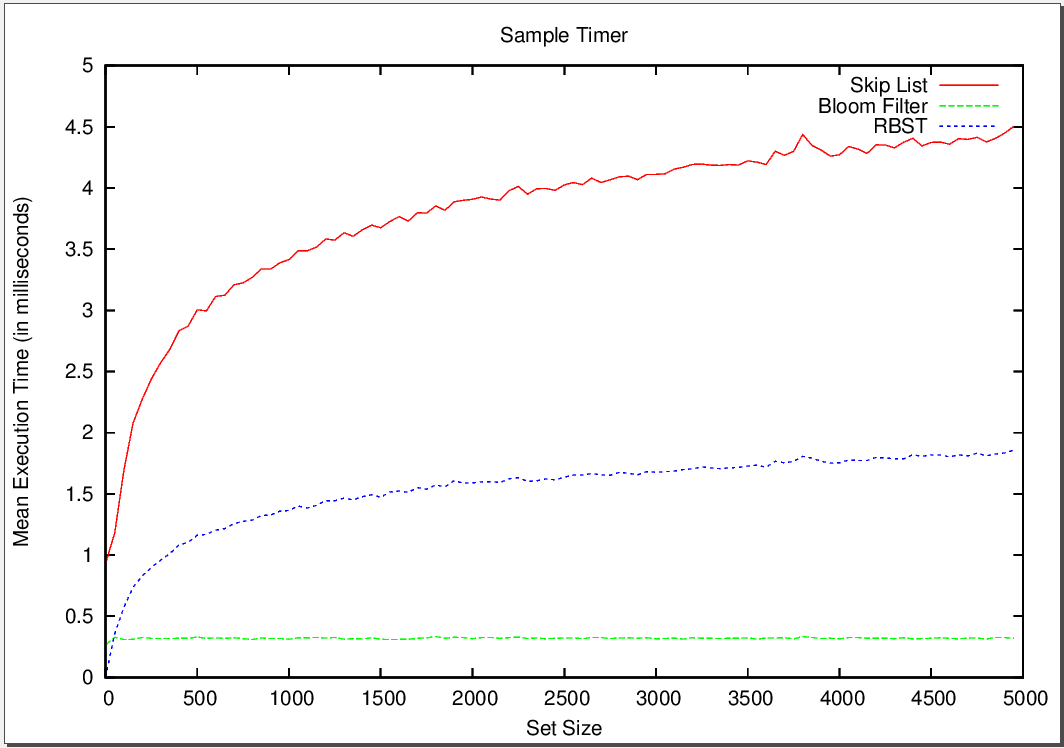
\includegraphics[height=70mm,width=100mm]{findtimer.png}
\caption{findtimer}
\end{figure}


\end{document}